\documentclass{beamer}
%\documentclass[trans]{beamer} %om te printen!
%\transglitter etc: kunt ge pas zien op Full Screen (Ctrl+L)
\usepackage{etex}
\usepackage{tikz}

\usepackage{graphicx,multicol}

\usepackage[all]{xy}
\usepackage{enumerate}

\usepackage{graphicx}
\usepackage{beamerouterthememiniframes, beamercolorthemeann,srcltx,hyperref}
\usepackage{amsmath,amsthm,amssymb}

\newcommand{\upuparrow}{\mathrel{\reflectbox{\rotatebox[origin=c]{90}{$\twoheadrightarrow$}}}}
\newcommand{\downdownarrow}{\mathrel{\reflectbox{\rotatebox[origin=c]{90}{$\twoheadleftarrow$}}}}
\setbeamercolor{normal text}{fg=black!70}
\setbeamertemplate{navigation symbols}{}%geen navigatie
\setbeamertemplate{blocks}[rounded][shadow=true]

%\setbeamercovered{dynamic} %te komen items in lichtgrijs
%\setbeamercolor{background canvas}{bg=black!0}%is wit

\logo{\vspace{-0.2cm}\\
\hfill
\includegraphics[height=3cm]{VUB_schild}}
%plaatst het logo op elke slide onderaan

\newcommand{\Z}{\mathbb{Z}}
\newcommand{\Q}{\mathbb{Q}}
\renewcommand{\P}{\mathbb{P}}
\newcommand{\R}{\mathbb{R}}
\newcommand{\N}{\mathbb{N}}
\newcommand{\C}{\mathbb{C}}
\newcommand{\U}{\mathcal{U}}
\newcommand{\E}{\mathbb{E}}
\newcommand{\z}{\mathcal{Z}}
\newtheorem{remark1}{Remark}
\newcommand{\LFP}{\text{LFP}}
%\columnsep=1.8cm %\columnseprule=.4pt
\newcommand{\cost}{\text{cost}}
\newcommand{\Nash}{\text{Nash}}
\newcommand{\nash}{\text{nash}}
\newcommand{\opt}{\text{opt}}
\newcommand{\copt}{\cost(a_{\opt})}
\title{The Scott Topology}
\author{Filip Moons\\3$^{\text{th}}$ Bachelor of Mathematics\\Promotor: Prof. Dr. Eva Colebunders\\Presentation Bachelor Thesis II}
\date{Friday 19 April, 2013}

\begin{document}

\begin{frame}[plain]

\includegraphics[width=0.4\paperwidth]{VUB_logo.jpg}
\vspace{2cm}
\titlepage
\end{frame}


%\section[Overzicht]{}%rechte haken dienen om niet in de outline te komen
%maar wel vanboven in het donkergroene balkje

%\begin{frame}[plain]{Outline}
%\end{frame}
%
%\begin{frame}[plain]{Outline}
%\tableofcontents[pausesections]
%\end{frame}
%
%
%\section{blabla}
%
%\begin{frame}
%\begin{alertblock}{}
%\begin{center}
%blabla
%\end{center}
%\end{alertblock}
%\end{frame}

\begin{frame}{Content}
\begin{itemize}
  \item Order theory
    \begin{itemize}
        \item Directed sets
        \item The ``Way Below''-relation
        \item Domains
    \end{itemize}
  \item Scott Convergence
    \begin{itemize}
        \item $\mathcal{S}$-limits
        \item Introducing the Scott topology
    \end{itemize}

  \item Scott-Continuous functions
   \begin{itemize}
        \item Definition
        \item Kleene Fixed Point Theorem
    \end{itemize}
  \item A categorical conclusion: injective spaces
\end{itemize}

\end{frame}


\section{Order theory}
\subsection{Ordered sets}
\begin{frame}{Preordered \& partially ordered sets}
\begin{block}{Definition: Directed sets}
Let $L$ be a preordered set. A subset $D$ of $L$ is directed provided it is nonempty and every finite subset of $D$ has an upper bound in $D$.
\end{block}
\begin{block}{Definition: Lower sets}
$$\downarrow X = \{y \in L: y \leq x \text{ for some } x \in X \}$$
X is an \emph{lower set} if $X = \downarrow X$.
\end{block}

\begin{block}{Definition: Dcpo}
A poset is complete with respect to directed sets if every directed set has supremum. A \textbf{dcpo} is a \textbf{d}irected \textbf{c}omplete \textbf{po}set.
\end{block}
\end{frame}
%\begin{frame}
%\begin{block}{}
%\begin{center}
%Introductie
%\end{center}
%\end{block}
%\end{frame}
\subsection{The ``Way Below''-relation}

\begin{frame}{The ``Way Below''-relation}


\begin{block}{Definition}
Let $L$ be a poset. $x$ is way below $y$, in symbols $x \ll y$, iff for all dircted subsets $D \subseteq L$, for which $\sup D$ exists, the relation $y \leq \sup D$ always implies the existence of a $d \in D$ with $x \leq d$.
\end{block}

\begin{block}{}
$$\downdownarrow x = \{u \in L: u \ll x\}$$
\end{block}
\end{frame}



\begin{frame}{The ``Way Below''-relation}
\begin{block}{Definition}
Let $L$ be a poset. $x$ is way below $y$, in symbols $x \ll y$, iff for all dircted subsets $D \subset L$, for which $\sup D$ exists, the relation $y \leq \sup D$ always implies the existence of a $d \in D$ with $x \leq d$.
\end{block}

\begin{block}{Example}
\begin{figure}
  \centering
  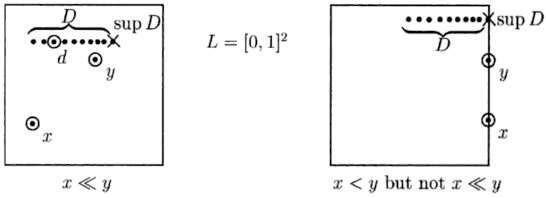
\includegraphics[scale=0.5]{figuurway.jpg}\\
\end{figure}
\end{block}


\end{frame}


\begin{frame}{The ``Way Below''-relation}


\begin{block}{Definition}
Let $L$ be a poset. $x$ is way below $y$, in symbols $x \ll y$, iff for all dircted subsets $D \subset L$, for which $\sup D$ exists, the relation $y \leq \sup D$ always implies the existence of a $d \in D$ with $x \leq d$.
\end{block}
\begin{block}{Example}
Let $X$ be a topological space and $\mathcal{O}(X)$ the complete lattice of open sets in $X$. Suppose $U, V \in \mathcal{O}(X)$ and define the order $\leq$ as the inclusion relation $\subseteq$.
\begin{align*}
 U \ll V \Leftrightarrow &\forall \mathcal{G} \text{ open cover of } V,\\
 &\exists \mathcal{G}' \subseteq \mathcal{G} \text{ finite cover of } U.
\end{align*}
\end{block}
\end{frame}

\subsection{Domains}
\begin{frame}{Domains}
\begin{block}{Definition: Continuous posets}
A poset $L$ is called \emph{continuous} if $\downdownarrow x$ is directed with supremum $x$ for all $x \in L$.
\end{block}

\begin{block}{Definition: Domain}
A dcpo which is continuous as a poset will be called a \emph{domain}.
\end{block}

\begin{block}{Example}
Let $M$ be a set and $L = 2^M$, then $2^M$ is a continuous lattice and thus a domain.
\end{block}
\end{frame}

\section{Scott convergence}
\subsection{$\mathcal{S}$-limits}
\begin{frame}{$\mathcal{S}$-limits on complete semilattices}
\begin{block}{Definition: Lower limit}
Let $L$ be a complete semilattice. For any net $(x_j)_{j\in J}$ we write
$$\liminf_j x_j = \sup_j \inf_{i \geq j} x_i,$$
and call $\liminf_j x_j$ the \emph{lower limit} or \emph{liminf} of the net.
\end{block}

\begin{block}{Definition: $\mathcal{S}$-limit}
Let $\mathcal{S}$ denote the class of the pairs $((x_j)_{j\in J}, x)$ such that $x \leq \liminf_j x_j$ ($\mathcal{S} = \{((x_j)_{j\in J}, x) | x \leq \liminf_j x_j \}$) . For each such pair we say that $x$ is an $\mathcal{S}-limit$ of $(x_j)_{j \in J}$ and we write briefly $x \equiv_{\mathcal{S}} \lim x_j$.
\end{block}
\end{frame}



\subsection{Convergence \& Topology}
\begin{frame}{The Scott Topology}
\begin{block}{Theorem: The general relation between convergence \& topology}
Let $\mathcal{L}$ be a class of pairs $((x_j)_{j\in J}, x)$ consisting of a net and an element of $L$, then
\begin{align*}
\mathcal{O}(\mathcal{L}) = \{&U \subseteq L | \text{ if } ((x_j)_{j\in J}, x) \in \mathcal{L} \text{ and } x \in U \text{ then eventually } \\
&x_j \in U\}
\end{align*}

is a topology.
\end{block}
\begin{block}{Definition: The Scott topology}
Take $\mathcal{L} = \mathcal{S}$, then $\mathcal{O}(\mathcal{S})$ is the \emph{Scott topology.}
\end{block}
\end{frame}

\begin{frame}{The Scott topology}
\begin{theorem}\label{scottprot} Let $L$ be dcpo and $U \subset L$. Then $U \in \mathcal{O}(\mathcal{S})$ iff the following two conditions are satisfied:
\begin{enumerate}[(i)]
    \item $U = \uparrow U$;
    \item $\sup D \in U$ implies $D \cap U \neq \emptyset$ for all directed set $D \subseteq L$.
\end{enumerate}
\end{theorem}

\end{frame}
\begin{frame}{The Scott topology}
\begin{block}{Example: the Sierpinski topology}
On the chain $L = \{0, 1\}$, the \emph{Scott topology} equals the \emph{Sierpinski topology.}
\end{block}
\begin{block}{Example: the unit interval}
If $L$ is the unit interval: $L = [0,1]$, then $L$ is a dcpo.  Any Scott open set has the form $]x,1]$ if $0 \leq x \leq 1$ or $[0, 1]$.
\end{block}
\end{frame}
\subsection{The Scott topology on domains}
\begin{frame}{The Scott topology on domains}
\begin{block}{Definition: Topological}
If $\mathcal{S}$ is precisely the class of convergent nets for the Scott topology, then we say that $\mathcal{S}$ is \emph{topological}.
\end{block}

\begin{theorem}
$$\mathcal{S}\text{-convergence is topological} \Leftrightarrow L \text{ is a domain}$$
\end{theorem}
\end{frame}

\section{Scott-continuous functions}
\subsection{Scott-continuous functions}
\begin{frame}{Definition}
\begin{theorem}
For a function $f: S \rightarrow T$, with $S,T$ dcpo's, the following conditions are equivalent:
\begin{enumerate}
    \item $f$ is continuous with respect to the Scott topologies, that is $$f^{-1}(U) \in \sigma(S),\; \forall U \in \sigma(T),$$
    \item f preserves suprema of directed sets, that is, $f$ is order preserving and $f(\sup D) = \sup f(D)$, for all directed subsets $D$ of $S$.
\end{enumerate}
\end{theorem}

\begin{block}{Definition: Scott-continuous}
A function $f: S \rightarrow T$ between dcpo's is \emph{Scott-continuous} iff it satisfies the equivalent conditions in the previous theorem.
\end{block}
\end{frame}
\subsection{Kleene Fixed-Point theorem}
\begin{frame}{Kleene Fixed-Point theorem}
\begin{block}{Theorem: Kleene Fixed-Point theorem} Let $L$ be a dcpo with a least element $\bot$, then it has the following properties:
\begin{enumerate}[(i)]
  \item \textbf{Existence}: Every Scott-continuous self-map $f: L \rightarrow L$ has a least fixed-point, notated by \LFP($f$).
  \item \textbf{Construction}: The least fixed-point can be approximated by the recursively defined \emph{Kleene chain}:
      $$x_0 = \bot, \; x_{n+1} = f(x_n) = f^{n+1}(\bot)$$
      in the sense that
      $$\text{\LFP}(f) = \sup_n x_n = \sup_n f^n(\bot).$$
\end{enumerate}
\end{block}

\end{frame}

\begin{frame}{Kleene Fixed-Point theorem}
\begin{block}{Example: The factorial function}
The definition of factorial as the function that maps $n \in \N$ to \texttt{f(n) = if $n$ = 0 then 1 else n.$f(n-1)$} is obtained as the least fixed point of the higher-order function $F$, mapping any function $f$ to the function $f'$ defined by \texttt{f($n$) = if $n$ = 0 then 1 else n.$f($n$-1)$}.
\end{block}
\end{frame}


\section{Injective spaces}
\subsection{Category theory}
\begin{frame}{Definitions}
\begin{block}{Category: $CONT$}
The category whose objects are \emph{continuous lattices} and whose morhpisms are \emph{Scott-continuous maps} will be denoted by $CONT$.
\end{block}

\begin{block}{Definition: $\Sigma$-functor}
Let $L$ be a continuous lattice, we call $\Sigma: CONT \rightarrow TOP$ the functor that associates to $L$ its Scott topology $\Sigma(L)$.
\end{block}

\end{frame}
\begin{frame}{Definitions}
\begin{block}{Definition: Specialization order}
The relation $$x\leq y \Longleftrightarrow x \in \overline{\{y\}}$$
is called the \emph{specialization order}.
\end{block}

\begin{block}{Definition: $\Omega$-functor}
We denote by $\Omega: TOP \to POSET$ the functor which associates with a space $X$ the poset $\Omega X = (X, \leq)$, where $\leq$ is the specialization order, and with $\Omega f = f$.
\end{block}

\end{frame}
\subsection{Injective spaces}
\begin{frame}
\begin{block}{Definition: Injective spaces}
A $T_0$-space $Z$ is called \emph{injective} iff every continuous map $f: X \rightarrow Z$ extends continuously to any space $Y$ containing $X$ as a subspace.
 \begin{center}
  \begin{tikzpicture}[node distance=2cm, auto]
  \node (Z) {$Z$};
  \node (X) [below of=Z] {$X$};
  \node (Y) [right of=X] {$Y$};
  \draw[->] (X) to node {$f$} (Z);
  \draw[>=latex,>->] (X) to node [swap] {j} (Y);
  \draw[->, dashed] (Y) to node [swap] {$f^*$} (Z);
\end{tikzpicture}
 \end{center}
\end{block}

\begin{block}{Category: $INJ$}
The category $INJ$ is the full subcategory of $TOP$ consisting of \emph{injective spaces} and all continuous maps.
\end{block}
\end{frame}
\subsection{Conclusion}
\begin{frame}
\begin{theorem}
\begin{enumerate}[(i)]
  \item If $L$ is a continuous lattice, then $\Sigma L = (L, \sigma(L))$ is an injective space and $\Omega\Sigma L = L$.
  \item If $X$ is an injective $T_0$-space, then $\Omega X = (X, \leq)$ is a continuous lattice (with respect to the specialization order) and $\Sigma\Omega X = X$.
\end{enumerate}
\end{theorem}

\end{frame}
\section{Bibliography}
\begin{frame}
\begin{block}{}
\begin{thebibliography}{99}
\bibitem{1} G. Gierz, K. H. Hofmann, K. Keimel, J. D. Lawson, M. W. Mislove, D. S. Scott, {\em Continuous Lattices and Domains}, Cambridge University Press, Cambridge (2003).
\bibitem{2} E. Colebunders, \emph{Topologie}, Vrije Universiteit Brussel, 2012.
\bibitem{3} K. Martin, \emph{A Foundation for Computation}, PhD thesis, Tulane University, Department of Math, July 2000
\bibitem{4} J.Goubault-Larrecq, \emph{Non-Hausdorff Topology and Domain Theory}, Cambridge University Press, 2013.
\bibitem{5} S. Abramsky, Dov M. Gabbay, T. S. E. Maibaum, \emph{Handbook for Logic in
Computer Science}, Clarendon Press Oxford, 1994.
    \end{thebibliography}
\end{block}
\end{frame}
\end{document}
